\documentclass[border=15pt, tikz]{standalone}
\usepackage{tikz}
\usetikzlibrary{positioning, arrows.meta, calc, backgrounds}

\begin{document}

% ==============================================================================
% ESTILOS REUTILIZABLES PARA DIAGRAMAS DE SECUENCIA (DRY)
% ==============================================================================
\pagecolor{white}
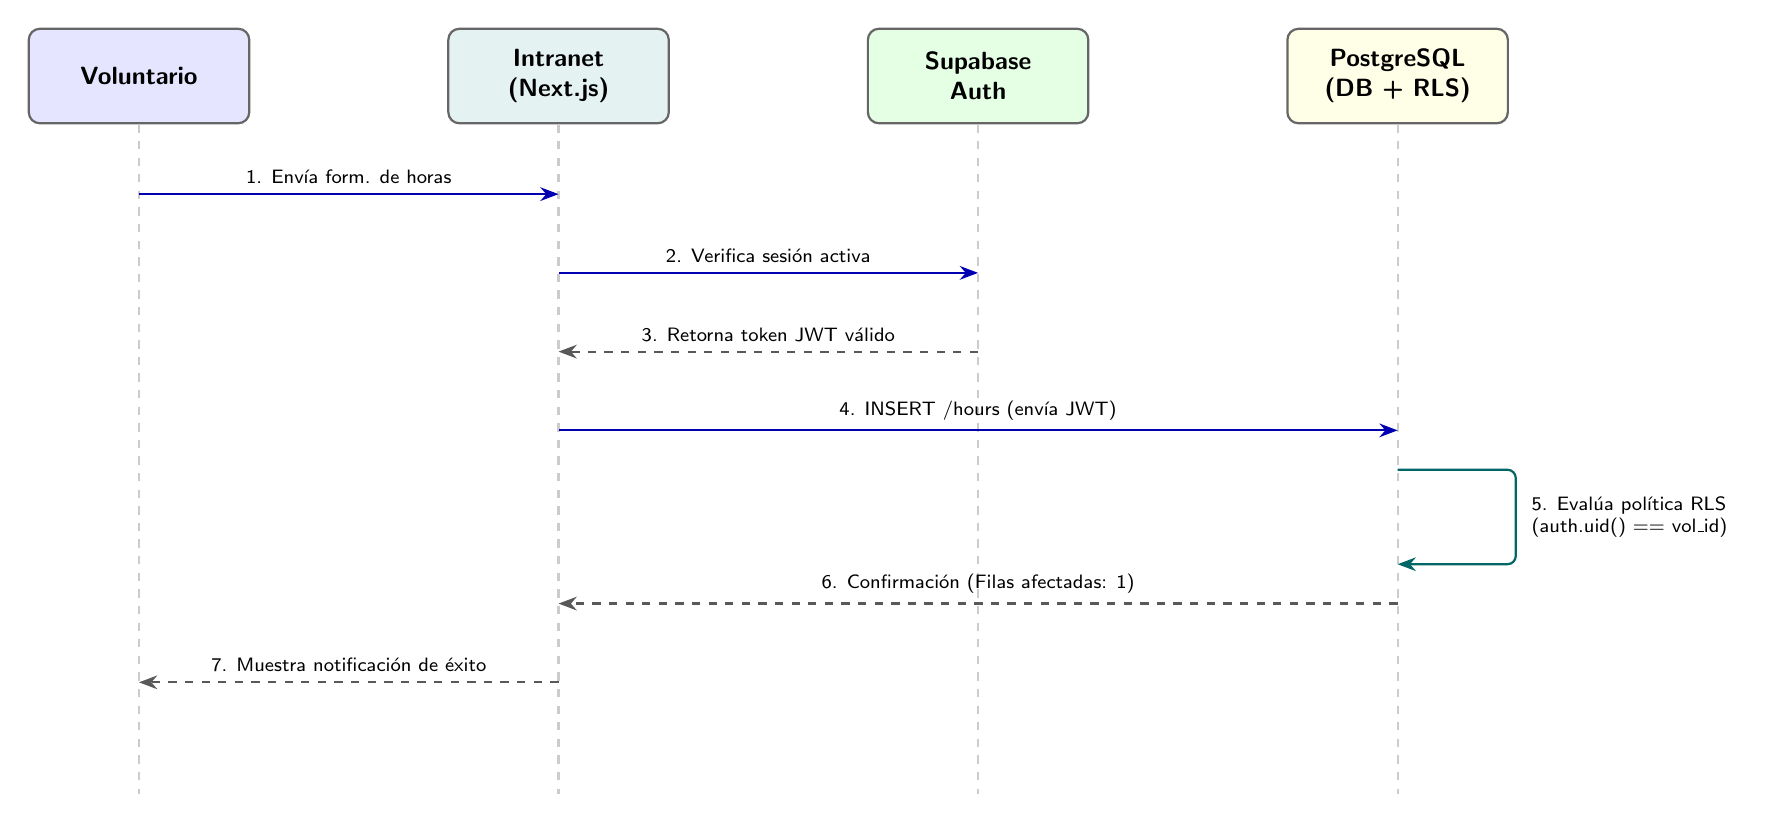
\begin{tikzpicture}[
    lifeline node/.style={
        draw=gray!80!black, fill=#1, rectangle, rounded corners,
        minimum width=2.8cm, minimum height=1.2cm, 
        font=\sffamily\small\bfseries, align=center, thick
    },
    msg/.style={->, >=Stealth, thick, draw=blue!70!black},
    ret/.style={->, >=Stealth, dashed, thick, draw=gray!70!black},
    self msg/.style={->, >=Stealth, thick, draw=teal!80!black, rounded corners=3pt},
    lbl/.style={above, font=\sffamily\scriptsize, align=center, text=black},
    lbl right/.style={right, font=\sffamily\scriptsize, align=left, text=black}
]

% Definición de la longitud de las líneas de vida
\def\len{8.5} 

% ------------------------------------------------------------------------------
% 1. PARTICIPANTES (Posicionamiento Relativo Eje X)
% ------------------------------------------------------------------------------
\node[lifeline node=blue!10] (vol) {Voluntario};
\node[lifeline node=teal!10, right=2.5cm of vol] (front) {Intranet\\(Next.js)};
\node[lifeline node=green!10, right=2.5cm of front] (auth) {Supabase\\Auth};
\node[lifeline node=yellow!10, right=2.5cm of auth] (db) {PostgreSQL\\(DB + RLS)};

% ------------------------------------------------------------------------------
% 2. LÍNEAS DE VIDA (Bucle DRY)
% ------------------------------------------------------------------------------
\foreach \x in {vol, front, auth, db} {
    \draw[thick, gray!40, dashed] (\x.south) -- ++(0,-\len);
}

% ------------------------------------------------------------------------------
% 3. MENSAJES (Posicionamiento Relativo Eje Y mediante intersecciones |-)
% ------------------------------------------------------------------------------
% Paso 1
\draw[msg] (vol |- 0,-1.5) -- node[lbl] {1. Envía form. de horas} (front |- 0,-1.5);

% Paso 2
\draw[msg] (front |- 0,-2.5) -- node[lbl] {2. Verifica sesión activa} (auth |- 0,-2.5);

% Paso 3
\draw[ret] (auth |- 0,-3.5) -- node[lbl] {3. Retorna token JWT válido} (front |- 0,-3.5);

% Paso 4
\draw[msg] (front |- 0,-4.5) -- node[lbl] {4. INSERT /hours (envía JWT)} (db |- 0,-4.5);

% Paso 5 (Mensaje a sí mismo / Proceso interno)
\draw[self msg] (db |- 0,-5.0) -- ++(1.5,0) |- node[lbl right, near start, xshift=2pt] {5. Evalúa política RLS\\(auth.uid() == vol\_id)} (db |- 0,-6.2);

% Paso 6
\draw[ret] (db |- 0,-6.7) -- node[lbl] {6. Confirmación (Filas afectadas: 1)} (front |- 0,-6.7);

% Paso 7
\draw[ret] (front |- 0,-7.7) -- node[lbl] {7. Muestra notificación de éxito} (vol |- 0,-7.7);

\end{tikzpicture}
\end{document}
